\documentclass[a4paper,10pt]{article}

\usepackage[hidelinks]{hyperref}
\usepackage{float}
\usepackage{tabularx}

% Lingua 
\usepackage[utf8]{inputenc}
\usepackage[italian]{babel}

% Margini
\usepackage{geometry}
\geometry{a4paper, top=3cm, bottom=3cm, left=3cm, right=3cm}
\setlength{\parindent}{0pt}

\usepackage{graphicx}   % per immagini
\usepackage{caption}    % per didascalie
\captionsetup[table]{labelformat=empty}
\usepackage{ifthen}     % per \ifthenelse
\usepackage{longtable}

\usepackage{array}      % per tabelle
\newcolumntype{M}[1]{>{\centering\arraybackslash}m{#1}}

\setcounter{secnumdepth}{5}
\setcounter{tocdepth}{5}
\usepackage{titlesec}

\titleformat{\paragraph}[block]  % <-- QUESTO è il punto chiave
  {\normalfont\normalsize\bfseries}
  {\theparagraph}
  {1em}
  {}

\titlespacing*{\paragraph}
  {0pt}
  {3ex}
  {1.5ex}

\usepackage{datetime}

% Definisci un formato personalizzato
\newdateformat{italianformat}{\THEDAY~\monthname[\THEMONTH]~\THEYEAR}
\newdate{dataverbale}{02}{04}{2026}

% Definizione del formato con le barre
\newdateformat{slashdate}{\twodigit{\THEDAY}/\twodigit{\THEMONTH}/\THEYEAR}

% Per logo in ogni pagina
\usepackage{eso-pic}
\usepackage{tikz}
\AddToShipoutPictureBG{%
  \ifthenelse{\value{page}>1}{%
    \begin{tikzpicture}[remember picture, overlay]
      % Icona
      \node[anchor=north west, inner sep=0pt] at ([xshift=28pt,yshift=-28pt]current page.north west) 
        {
\includegraphics[width=1cm, height=1cm]{resources/Tool-8_icon_white.png}};
      
      % Riga
      \draw[black, line width=0.5pt] ([xshift=28pt + 1cm, yshift=-28pt - 0.6cm]current page.north west) 
            -- ++(3.2cm, 0);
      % Testo
      \node[anchor=west, text=black, font=\small] at ([xshift=28pt + 1cm, yshift=-28pt - 0.4cm]current page.north west) 
        {Specifica Tecnica};
    \end{tikzpicture}
  }{}
}

% Nome indice figure
\addto\captionsitalian{%
  \renewcommand{\listfigurename}{Indice delle immagini}%
}


%------Ridefinizione maketitle-------
\makeatletter
\renewcommand{\maketitle}{%
  \vspace*{\fill}
  \begin{center}
    {\LARGE \bfseries \@title \par}
    \vskip 1em
    {\large \@author \par}
    \vskip 1em
    {\large\slashdate{\displaydate{dataverbale}} \par}
  \end{center}
  \vspace*{\fill}
}
\makeatother
%-----------------------------------

\title{%
  
\includegraphics[width=10cm]{resources/Tool-8_white_2.png} \\[1.5ex]
  \textbf{\LARGE Specifica Tecnica}
}
\author{}
\date{\dataverbale}
\begin{document}
\tikz[remember picture,overlay] \node[opacity=0.2,inner sep=0pt] at (current page.center){
\includegraphics[width=\paperwidth,height=\paperheight]{resources/Abstract_lines.png}};

\maketitle

\newpage

\section*{Revisioni}
\begin{table}[h!]
\centering
\begin{tabular}{|M{0.8cm}|p{2.2cm}|p{5.7cm}|M{1.8cm}|p{2.2cm}|}
  \hline
  \textbf{Ver.} & \textbf{Autore} & \textbf{Modifiche} & \textbf{Data} & \textbf{Verifica} \\
  \hline
  0.2 & Stefano Maso & Stesura sezione 3.1, 3.1.1 e sottosezioni relative all'architettura del backend e relativi diagrammi delle classi & 08/04/2026 & Besnik Murtezan \\
  \hline
  0.1 & Giuliano Banchieri & Prima stesura: struttura del documento, tecnologie, riferimenti, introduzione & 02/04/2026 & Niccolò Feltrin \\
  \hline
\end{tabular}
\caption{}
\label{tab:revisioni}
\end{table}

\newpage

\tableofcontents

\newpage

\listoffigures

\newpage

\section{Introduzione}
\subsection{Scopo del documento}
Il presente documento contiene informazioni dettagliate sulle tecnologie utilizzate e sulle scelte progettuali del gruppo Tool-8 per la realizzazione del prodotto \textbf{Second Brain} su richiesta dell'azienda \textbf{Zucchetti S.p.A.}

Sono fornite descrizioni delle tecnologie scelte per backend, frontend e di supporto, i diagrammi delle classi che rappresentano in modo dettagliato l'archittettura logica e una tabella di tracciamento dei requisiti soddisfatti.

\subsection{Scopo del prodotto}
"\textbf{Estendere il note-taking con i Large Language Models.}"

L'obiettivo del capitolato C6 "\textbf{Second Brain}" è lo sviluppo di un applicativo che fornisca all'utente un editor di file MD con funzionalità AI che semplifichino la scrittura tramite funzionalità come: riassunto, traduzione, critica, correzione, e generazione del testo.

L'utente avrà la possibilità di utilizzare queste funzionalità anche tramite interrogazioni in linguaggio naturale che verranno processate da un LLM contattato dal sistema.

Il software sarà sviluppato sotto forma di applicazione web dove l'utente potrà creare, salvare, eliminare e modificare le sue note.

\subsection{Riferimenti}
\subsubsection{Riferimenti normativi}
\begin{itemize}
  \item Capitolato C6 - Progetto Second Brain: \\  \url{https://www.math.unipd.it/~tullio/IS-1/2025/Progetto/C6.pdf}
  \item Regolamento progetto didattico: \\ \url{https://www.math.unipd.it/~tullio/IS-1/2025/Dispense/PD1.pdf}
  \item \href{https://tool-8.github.io/Documentazione-SWE/pb/Norme_di_Progetto_v1.1.pdf}{Norme di Progetto v1.1}
  \item \href{https://tool-8.github.io/Documentazione-SWE/pb/Analisi_dei_Requisiti_v1.5.pdf}{Analisi dei Requisiti v1.5}
\end{itemize}
\subsubsection{Riferimenti informativi}
\begin{itemize}
  \item \href{https://tool-8.github.io/Documentazione-SWE/}{Verbali}
  \item \href{https://tool-8.github.io/Documentazione-SWE/glossario/Glossario.pdf}{Glossario v1.0}
  \item Lezioni del corso di \textit{Ingegneria del software} aggiornate al 02/04/2026:
  \begin{itemize}
    \item \textit{"Progettazione software (T6)"}: \\ \url{https://www.math.unipd.it/~tullio/IS-1/2025/Dispense/T06.pdf}
    \item \textit{"Progettazione e programmazione: Diagrammi delle classi (UML)"}: \\ \url{https://www.math.unipd.it/~rcardin/swea/2023/Diagrammi%20delle%20Classi.pdf}
    \item \textit{"Analisi e descrizione delle funzionalità: Diagrammi delle attività (UML)"}: \\ \url{https://www.math.unipd.it/~rcardin/swea/2022/Diagrammi%20di%20Attivit%C3%A0.pdf}
    \item \textit{"Progettazione: I pattern architetturali"}: \\ \url{https://www.math.unipd.it/~rcardin/swea/2022/Software%20Architecture%20Patterns.pdf}
    \item \textit{"Progettazione: Il pattern Dependency Injection"}: \\ \url{https://www.math.unipd.it/~rcardin/swea/2022/Design%20Pattern%20Architetturali%20-%20Dependency%20Injection.pdf}
    \item \textit{"Progettazione: Pattern Architetturali per le applicazioni con UI"}: \\ \url{https://www.math.unipd.it/~rcardin/sweb/2022/L02.pdf}
    \item \textit{"Progettazione: i pattern creazionali (GoF)"}: \\ \url{https://www.math.unipd.it/~rcardin/swea/2022/Design%20Pattern%20Creazionali.pdf}
    \item \textit{"Progettazione: I pattern strutturali (GoF)"}: \\ \url{https://www.math.unipd.it/~rcardin/swea/2022/Design%20Pattern%20Strutturali.pdf}
    \item \textit{"Progettazione: I pattern di comportamento (GoF)"}: \\ \url{https://drive.google.com/file/d/1cpi6rORMxFtC91nI6_sPrG1Xn-28z8eI/view?usp=sharing}
    \item \textit{"Programmazione: SOLID programming}: \\ \url{https://drive.google.com/file/d/1o1Xun2dVVc3mDiaGyN0FrDJhhoO3lfLQ/view?pli=1}
  \end{itemize}
\end{itemize}

\newpage

\section{Tecnologie}
In questa sezione sono descritte le tecnologie utilizzate per lo sviluppo di \textbf{Second Brain}.

Sono inclusi gli strumenti, i framework e le librerie utilizzati per lo sviluppo di backend, frontend e della parte di persistenza dei dati ma anche quelli di supporto, di verifica e i servizi esterni.
\subsection{Tecnologie di codifica}
Framework e librerie utilizzate per lo sviluppo backend e frontend.

\subsubsection{TypeScript}
TypeScript è un linguaggio basato su JavaScript che introduce la tipizzazione statica, migliorando la manutenibilità e la robustezza del codice.
\begin{itemize}
    \item \textbf{Versione}:
    \item \textbf{Documentazione}: \url{https://www.typescriptlang.org/docs/}
\end{itemize}

\subsubsection{Vue.js}
Vue è un framework open source per lo sviluppo di interfacce utente e single-page-application. Si basa su HTML, CSS, e JavaScript e fornisce un modello di programmazione dichiarativa basato su componenti che aiuta l'utilizzatore a costruire interfacce reattive di qualsiasi complessità.
\begin{itemize}
    \item \textbf{Versione}:
    \item \textbf{Documentazione}: \url{https://vuejs.org/guide/introduction.html}
\end{itemize}

\subsubsection{Marked.js}
Marked.js è una libreria open-source scritta in JavaScript utilizzata per il parsing e la conversione di testo in formato Markdown. Consente di trasformare contenuti Markdown in HTML in modo rapido, supportando estensioni personalizzate e integrazione lato client e server.
\begin{itemize}
    \item \textbf{Versione}:
    \item \textbf{Documentazione}: \url{https://marked.js.org/}
\end{itemize}

\subsubsection{CSS}
CSS (Cascading Style Sheets) è un linguaggio utilizzato per la formattazione di documenti HTML, XHTML e XML.
\begin{itemize}
    \item \textbf{Versione}:
    \item \textbf{Documentazione}: \url{https://developer.mozilla.org/en-US/docs/Web/CSS}
\end{itemize}

\subsubsection{Tailwind CSS}
Tailwind CSS è un framework CSS open source. Offre una serie  di classi CSS "di utilità". Queste classi vengono poi personalizzate e combinate seconde necessità per definire lo stile di ogni elemento.
\begin{itemize}
    \item \textbf{Versione}:
    \item \textbf{Documentazione}: \url{https://tailwindcss.com/docs/installation/using-vite}
\end{itemize}

\subsubsection{HTML}
HTML (HyperText Markup Language) è il linguaggio di markup più utilizzato al mondo per i documenti web. È un linguaggio di pubblico dominio e le sue regole sono dettate da \textbf{W3C} (World Wide Web Consortium)
\begin{itemize}
    \item \textbf{Versione}: HTML5
    \item \textbf{Documentazione}: \url{https://developer.mozilla.org/en-US/docs/Web/HTML}
\end{itemize}

\subsubsection{PHP}
PHP è un linguaggio di programmazione lato server progettato per lo sviluppo web, utilizzato per implementare la logica lato backend.
\begin{itemize}
    \item \textbf{Versione}:
    \item \textbf{Documentazione}: \url{https://www.php.net/manual/it/}
\end{itemize}

\subsubsection{Laravel}
Laravel è un framework open source scritto in PHP utilizzato per lo sviluppo di applicazioni web moderne. Adotta il pattern architetturale MVC (Model View Controller) e fornisce strumenti integrati per la gestione del routing, dell’autenticazione e dell’accesso ai dati.
\begin{itemize}
    \item \textbf{Versione}:
    \item \textbf{Documentazione}: \url{https://laravel.com/docs/13.x}
\end{itemize}


\subsection{Tecnologie di verifica}
Strumenti utilizzati per l'analisi del codice prodotto.

\subsubsection{PHPUnit}
PHPUnit è un framework utilizzato per l'analisi del codice PHP tramite test di unità. Lo scopo è trovare eventuali errori introdotti con modifiche al codice ed evitare che si verifichi una regressione.
\begin{itemize}
    \item \textbf{Versione}:
    \item \textbf{Documentazione}: \url{https://phpunit.de/documentation.html}
\end{itemize}

\subsection{Tecnologie per la persistenza dei dati (OPT)}

\subsubsection{PostgreSQL}
PostgreSQL è un sistema di gestione di database relazionali open source compatibile con i sistemi operativi più diffusi.
\begin{itemize}
    \item \textbf{Versione}:
    \item \textbf{Documentazione}: \url{https://www.postgresql.org/docs/}
\end{itemize}

\subsection{Tecnologie di supporto}
Strumenti utilizzati per facilitare lo sviluppo del prodotto da parte del gruppo.

\subsubsection{Vite}
Vite è uno strumento di sviluppo frontend che funge da dev server e build tool.
\begin{itemize}
    \item \textbf{Versione}:
    \item \textbf{Documentazione}: \url{https://vite.dev/guide/}
\end{itemize}

\subsubsection{Composer}
Composer è un gestore di dipendenze per il linguaggio PHP utilizzato per installare, aggiornare e gestire automaticamente librerie e pacchetti necessari a un progetto.
\begin{itemize}
    \item \textbf{Versione}:
    \item \textbf{Documentazione}: \url{https://getcomposer.org/doc/}
\end{itemize}

\subsubsection{nginx}
nginx è un web server open source leggero e ad alte prestazioni, utilizzabile anche come reverse proxy, load balancer, cache HTTP.
\begin{itemize}
    \item \textbf{Versione}:
    \item \textbf{Documentazione}: \url{https://nginx.org/en/docs/}
\end{itemize}

\subsubsection{PHP-FPM}

\begin{itemize}
    \item \textbf{Versione}:
    \item \textbf{Documentazione}: \url{https://www.php.net/manual/en/install.fpm.php}
\end{itemize}

\subsubsection{Docker}
Docker è una piattaforma di containerizzazione che consente di creare, distribuire ed eseguire applicazioni all’interno di ambienti isolati e leggeri, detti container. Ogni container include tutte le dipendenze necessarie al funzionamento del software ed è gestito in modo indipendente rispetto agli altri.
\begin{itemize}
    \item \textbf{Versione}:
    \item \textbf{Documentazione}: \url{https://docs.docker.com/}
\end{itemize}

\subsubsection{Docker Compose}
Docker Compose è uno strumento che consente di definire, configurare e gestire applicazioni multi-container. Permette di gestire l’avvio, l’arresto e l’interazione tra più container in modo coordinato.
\begin{itemize}
    \item \textbf{Versione}:
    \item \textbf{Documentazione}: \url{https://docs.docker.com/compose/}
\end{itemize}

\subsection{Modelli LLM esterni}
Large Language Models utilizzati per le funzionalità AI richieste

\subsubsection{...}

\newpage

\section{Architettura}
In questa sezione è descritta in modo dettagliato l'architettura del nostro prodotto. Verranno illustrate le nostre scelte progettuali e i componenti del nostro sistema.

\subsection{Architettura logica}
Il progetto Second Brain è strutturato in due componenti principali:
\begin{itemize}
    \item \textbf{Backend}: responsabile della gestione della \textit{logica di business} e della persistenza dei dati.
    \item \textbf{Frontend}: destinato alla presentazione dei dati ottenuti dal \textit{backend}, il \textit{frontend} consente all'utente di interagire con le funzionalità del progetto in modo intuitivo e user-friendly.
\end{itemize}
\subsubsection{Backend}
Nel \textit{backend} si è scelto di utilizzare il framework Laravel, che permette la realizzazione di un servizio API REST. L'architettura del backend è suddivisa nei seguenti strati: 
\begin{itemize}
    \item \textbf{Presentation Layer}: si occupa del routing delle richieste; i controller fungono da intermediari tra il client e i servizi, gestendo il presentation layer e instradando le richieste del client ai servizi appropriati.
    \item \textbf{Application Layer}: gestisce la \textit{logica di business} dell'applicazione; questo strato è responsabile delle operazioni e delle regole di business, garantendo che tutte le operazioni siano eseguite correttamente;
    \item \textbf{Data Access Layer}: strato che gestisce la persistenza dei dati, fornendo i mezzi per salvare, recuperare e manipolare i dati.
\end{itemize}
La suddivisione in questi strati facilita lo sviluppo, la manutenzione e la scalabilità del \textit{backend} del progetto Second Brain, conformandosi all'architettura \textbf{multi-tier} a 3-tier. 
\paragraph{Gestione note e Esportazione}
\vspace{0.5em}
\begin{figure}[H]
    \centering
    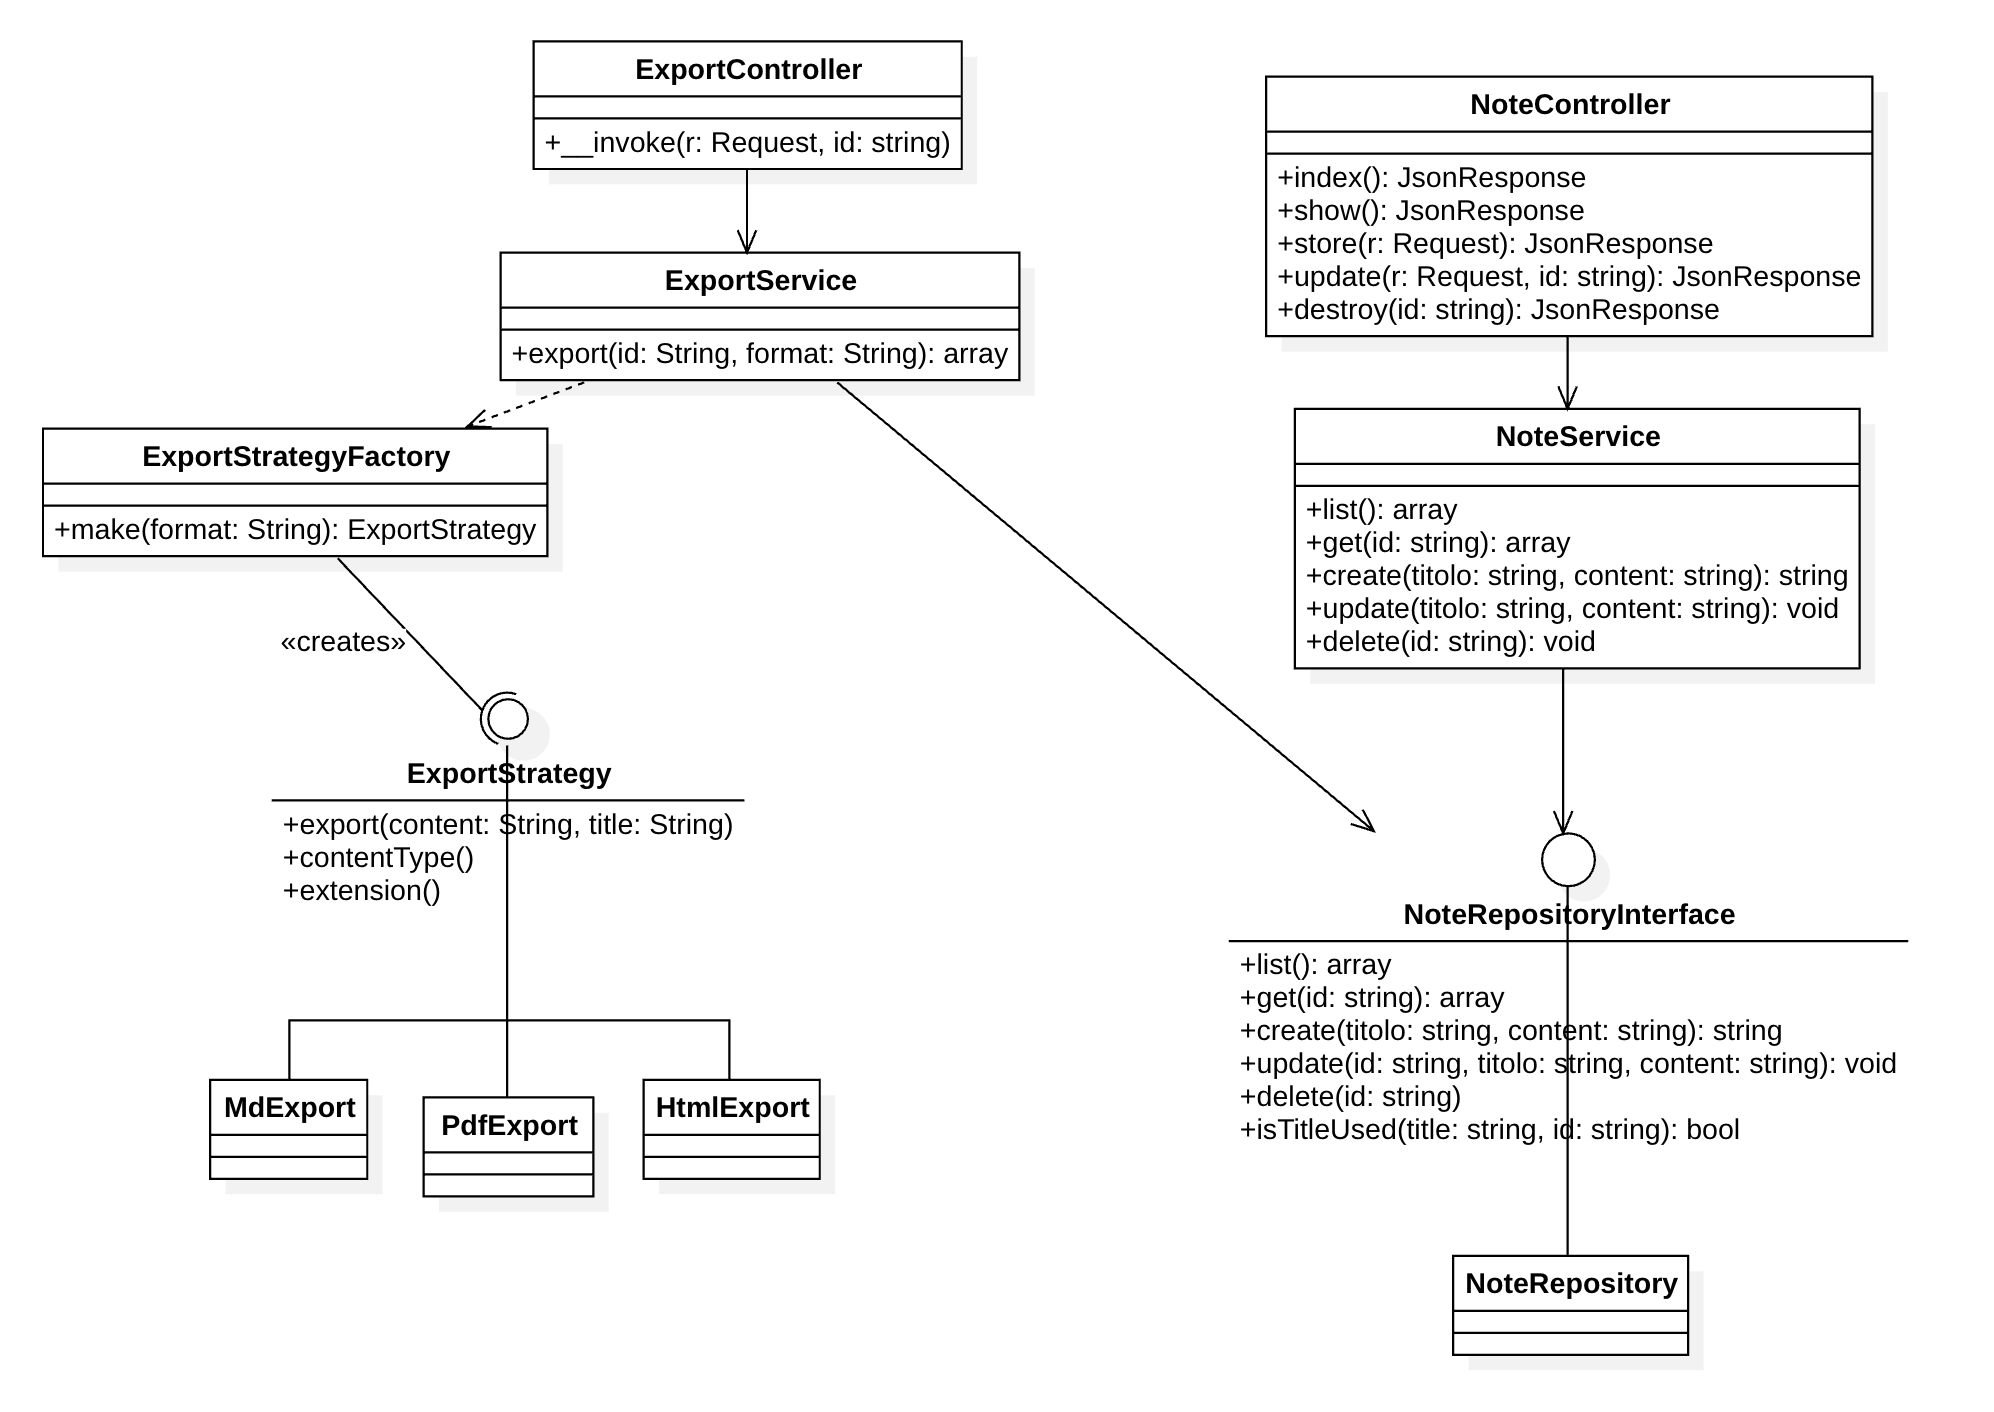
\includegraphics[width=1\textwidth]{resources/Gestione note e Esportazione.png}
    \caption{Diagramma delle classi per Gestione note e Esportazione}
    \label{fig:esempio}
\end{figure}
\subparagraph{NoteController}
È il controller HTTP responsabile della gestione delle richieste REST relative alle note. Appartiene al layer di presentazione dell'architettura layered e funge da punto di ingresso per tutte le operazioni CRUD esposte dall'API. Si limita a validare i dati in ingresso, delegare l'elaborazione a \textit{NoteService} e restituire una risposta HTTP appropriata. Segue la descrizione dei metodi:
\begin{itemize}
    \item \texttt{index() : JsonResponse} - gestisce le richieste \texttt{GET /notes}, restituendo la lista completa delle note in formato JSON con status 200, delegando il recupero dei dati a NoteService
    \item  \texttt{show(string \$id) : JsonResponse} - gestisce le richieste \texttt{GET /notes/\{id\}} e restituisce i dettagli di una singola nota identificata dall'id fornito
    \item  \texttt{store(Request \$request) : JsonResponse} -  gestisce le richieste \texttt{POST /notes}, valida i campi, delega a NoteService la creazione e restituisce la nota creata con status 201
    \item \texttt{update(Request \$request, string \$id) : JsonResponse} - gestisce le richieste \texttt{PUT /notes/\{id\}}, valida i campi e delega l'aggiornamento a NoteService, passando l'id e i nuovi dati
    \item \texttt{destroy(string \$id) : JsonResponse} - gestisce le richieste \texttt{DELETE /notes/\{id\}}, delega l'eliminazione a NoteService e restituisce una risposta vuota con status 204 in caso di successo
\end{itemize}
\subparagraph{NoteService} È il service responsabile della logica di business relativa alle note. Appartiene al layer applicativo dell'architettura layered e funge da intermediario tra il controller e il repository. Dipende esclusivamente dall'interfaccia NoteRepositoryInterface, garantendo il rispetto del principio di inversione delle dipendenze. Segue la descrizione dei metodi:
\begin{itemize}
    \item \texttt{list() : array} - restituisce la lista completa delle note, delegando direttamente al repository
    \item \texttt{get(string \$id) : array} - restituisce i dettagli di una singola nota tramite il suo id
    \item \texttt{create(string \$title, string \$contentMd) : array} - gestisce la creazione di una nuova nota, verificando che il titolo non sia già in uso prima di delegare al repository 
    \item \texttt{update(string \$id, string \$title, string \$contentMd) : array} - gestisce l'aggiornamento di una nota esistente; prima di delegare al repository verifica che il titolo non sia già in uso, escludendo dal confronto la nota corrente così che una nota possa essere salvata con il proprio titolo invariato senza incorrere in un falso positivo
    \item \texttt{delete(string \$id) : void} - delega l'eliminazione della nota al repository
\end{itemize}
\subparagraph{NoteRepositoryInterface} Interfaccia che definisce il contratto che ogni implementazione del repository di note deve rispettare. Appartiene al layer di accesso ai dati dell'architettura layered. Dichiarando la dipendenza su questa interfaccia, NoteService può funzionare con qualsiasi implementazione senza richiedere modifiche al codice applicativo. Segue la descrizione dei metodi: 
\begin{itemize}
    \item \texttt{list() : array} - restituisce la lista completa delle note disponibili, ogni elemento dell'array contiene i metadati della nota senza il contenuto completo
    \item \texttt{get(string \$id) : array} - restituisce i dati completi di una singola nota identificata dall'id fornito
    \item \texttt{create(string \$title, string \$contentMd) : array} - crea una nuova nota con il titolo e il contenuto Markdown forniti, genera un identificatore e registra il timestamp di creazione
    \item \texttt{update(string \$id, string \$title, string \$contentMd) : array} - aggiorna il titolo e il contenuto di una nota esistente assieme al timestamp di ultima modifica
    \item \texttt{delete(string \$id) : void} - elimina definitivamente la nota identificata dall'id fornito
    \item \texttt{isTitleUsed(string \$title, ?string \$excludeId = null) : bool} - verifica se un titolo è già utilizzato da un'altra nota; \texttt{excludeId} permette di escludere dal confronto una nota specifica, per evitare che tale nota venga bloccata dal confronto con se stessa
\end{itemize}
\subparagraph{NoteRepository} È l'implementazione concreta di NoteRepositoryInterface che persiste le note come file Markdown sul filesystem locale tramite Laravel Storage. Realizza tutti i metodi dichiarati nell'interfaccia: \texttt{list(), get(), create(), update(), delete(), isTitleUsed()}; per la descrizione della firma e del contratto di ciascun metodo si rimanda alla sezione dedicata all'interfaccia.
\subparagraph{ExportController} È il controller HTTP responsabile della gestione delle richieste di esportazione, rendendo disponibile una nota come file scaricabile. Appartiene al layer di presentazione dell'architettura layered ed è implementato come controller invocabile dato che la sua responsabilità è circoscritta ad una sola operazione. Si limita a validare il formato richiesto, delega l'esportazione a \textit{ExportService} e costruisce la risposta HTTP con gli header appropriati per il download dei file. Segue la descrizione dei metodi:
\begin{itemize}
    \item \texttt{\_\_invoke(Request \$request, string \$id)} - valida il parametro (cioè il formato con cui si vuole esportare la nota) e delega l'esportazione a \textit{ExportService}, passando l'id della nota e il formato richiesto; in caso di successo restituisce una risposta binaria in modo che il browser tratti la risposta come un file da scaricare, altrimenti ritorna una risposta JSON con status 404
\end{itemize}
\subparagraph{ExportService} È il service responsabile della logica di esportazione di una nota in un formato file. Appartiene al layer applicativo dell'architettura layered e gestisce la collaborazione tra il repository e la factory delle strategy di esportazione. Dipende da NoteRepositoryInterface, garantendo il disaccopiamento dal layer di persistenza. Segue la descrizione dei metodi:
\begin{itemize}
    \item \texttt{export(string \$id, string \$format) : array} - recupera la nota identificata dall'id tramite il repository, delega la creazione della strategy corretta a \textit{ExportStrategyFactory} in base al formato richiesto ed invoca sulla strategy i diversi metodi per ottenere il contenuto del file esportato, il MIME type e l'estensione
\end{itemize}
\subparagraph{ExportStrategyFactory} È la factory responsabile della creazione della strategy di esportazione corretta in base al formato richiesto. Appartiene al layer applicativo dell'architettura layered e implementa il pattern Factory Method, centralizzando la logica di selezione della strategy. Segue la descrizione dei metodi:
\begin{itemize}
    \item \texttt{make(string \$format) : ExportStrategyInterface} - metodo statico che istanzia e restituisce la strategy concreta corrispondente al formato richiesto
\end{itemize}
\subparagraph{ExportStrategyInterface} Interfaccia che definisce il contratto che ogni strategy di esportazione deve rispettare. Appartiene al layer applicativo dell'architettura layered e rappresenta il punto di astrazione del pattern strategy applicato all'esportazione delle note. Segue la descrizione dei metodi:
\begin{itemize}
    \item \texttt{export (string \$content, string \$title) : string} - trasforma il contenuto Markdown della nota nel formato di output specifico della strategy
    \item \texttt{contentType() : string} - restituisce il MIME type associato al formato di esportazione, per consentire al browser di interpretare correttamente il file ricevuto
    \item \texttt{extension() : string} - restituisce l'estensione del file associata al formato di esportazione, utilizzata per costruire il nome del file
\end{itemize}
\subparagraph{MdExport} È l'implementazione concreta di ExportStrategyInterface per l'esportazione nel formato Markdown, è la strategy più semplice del sistema in quanto il contenuto delle note è già nativamente in formato Markdown, quindi non richiede alcuna trasformazione. Per la descrizione della firma e del contratto di ciascun metodo si rimanda alla sezione dedicata all'interfaccia.
\subparagraph{HtmlExport} È l'implementazione concreta di ExportStrategyInterface per l'esportazione nel formato HTML. Utilizza la libreria Parsedown per convertire il contenuto Markdown della nota in markup HTML, che viene poi incorporato in un documento HTML completo e ben formato. Per la descrizione della firma e del contratto di ciascun metodo si rimanda alla sezione dedicata all'interfaccia.
\subparagraph{PdfExport} È l'implementazione concreta di ExportStrategyInterface per l'esportazione nel formato PDF. Prima delega a \textit{HtmlExport} la trasformazione del Markdown in HTML, poi utilizza la libreria \texttt{barryvdh/laravel-domppdf} per convertire l'HTML in un documento PDF binario. Per la descrizione della firma e del contratto di ciascun metodo si rimanda alla sezione dedicata all'interfaccia.

\paragraph{Interazione con LLM}

\subsection{Architettura di deployment}

\subsection{Architettura di dettaglio}

\newpage

\section{Stato dei requisiti funzionali}
\begin{center}
    \begin{longtable}{|>{\centering\arraybackslash}m{2.5cm}|>{\centering\arraybackslash}m{8cm}|>{\centering\arraybackslash}m{2.5cm}|}
        \hline
        \textbf{Requisito} & \textbf{Descrizione} & \textbf{Rispettato} \\ \hline
        \endfirsthead
        \hline
        RF-O-1 & Il sistema deve permettere all’utente di visualizzare l’archivio delle note presenti e per ogni nota il suo nome, la data di creazione e la data dell’ultima modifica & NO \\ \hline
        \caption{}
    \end{longtable}
\end{center}

\end{document}

